% HINT: add option aspectratio=169 for 16:9 aspect ratio
% HINT: add 'handout' to activate handout mode (without overlays for printing)
\documentclass[t,english,aspectratio=169,handout]{beamer}
\setbeamerfont{frametitle}{family=\rmfamily }
\usepackage[backend=biber,style=authoryear,maxnames=2]{biblatex}
% include package import and macro defintions
% Math
\usepackage{amsmath}
\usepackage{upgreek}

% Miscelaneous
\usepackage{pgfpages}
\usepackage{csquotes}
\usepackage{placeins}
\usepackage[onehalfspacing]{setspace}

% Captions
\usepackage[labelformat=empty]{caption}

% Colors
\usepackage{xcolor}

% Requirements
\RequirePackage{tikz}
\usetikzlibrary{calc}
\usetikzlibrary{arrows,shapes,positioning}

% For \smiley{} and \frowney{}
\usepackage{wasysym}

% Pseudocode
\usepackage[vlined, linesnumbered, ruled]{algorithm2e}
\SetKwComment{Comment}{/* }{*/}
\SetKwInput{KwData}{Input}
\SetKwInput{KwResult}{Output}
\IncMargin{1.5em}

% nice icons
%\usepackage{fontawesome}

% IMPORTANT NOTE: outputdir needs to be equal to output/aux dir of xelatex
%\usepackage[outputdir=output]{minted}
\usepackage{appendixnumberbeamer}

% Tables
\usepackage{booktabs}
\usepackage{multicol}
\usepackage{multirow}
\usepackage{colortbl}

% Date formatting
\usepackage[short,nodayofweek]{datetime}

% Für Vektoren
\newcommand{\myvec}[1]{\ensuremath{\begin{pmatrix}#1\end{pmatrix}}}
\def\spvec#1{\left(\vcenter{\halign{\hfil$##$\hfil\cr \spvecA#1;;}}\right)}
\def\spvecA#1;{\if;#1;\else #1\cr \expandafter \spvecA \fi}

% Hyperlinks
\definecolor{citeblue}{rgb}{0,0.3,0.55}
\RequirePackage{hyperref}
\hypersetup{colorlinks,linkcolor={lightgray},citecolor={citeblue},urlcolor={citeblue}}
\let\oldciteauthor=\citeauthor
\def\citeauthor#1{\hypersetup{citecolor=white}\oldciteauthor{#1}}

% Added
\usepackage{circuitikz}
\usepackage{grfext}


% Custom Makros
\newcommand{\bangle}[1]{\langle #1 \rangle}
\newcommand{\semsof}[1]{\ensuremath{\llbracket #1 \rrbracket}}
\newcommand{\impl}{\Rightarrow}
\newcommand{\reason}[1]{\qquad \mid #1}
\newcommand{\edge}{\ensuremath{(e,e')}}
\newcommand{\edgein}{\ensuremath{(e,e') \in }}
\newcommand{\egdein}{\ensuremath{(e',e) \in }}
\newcommand{\defof}{\text{Def. of }~}
\newcommand{\inv}{\ensuremath{{-1}}}
\newcommand{\prf}{\mathcal{P}}
\newcommand{\catprf}{\ensuremath{\mathcal{P}^{CAT}}}
\newcommand{\I}{\mathcal{I}}

% Reelle, Natürliche, Ganze, Rationale Zahlen
\newcommand{\R}{\ensuremath{\mathbb{R}}}
\newcommand{\N}{\ensuremath{\mathbb{N}}}
\newcommand{\Z}{\ensuremath{\mathbb{Z}}}
\newcommand{\Q}{\ensuremath{\mathbb{Q}}}
\newcommand{\E}{\ensuremath{\mathbb{E}}}
\newcommand{\B}{\ensuremath{\mathfrak{B}}}
\newcommand{\C}{\ensuremath{\mathfrak{C}}}


% Kürzel für Basisrelationen
\definecolor{rfgreen}{rgb}{0.2,0.55,0.2}
\newcommand{\0}{\textsf{\upshape 0}} % \upshape ensures that the relations remain their look in lemmata and inferrules
\newcommand{\po}{\textsf{\upshape po}}
\newcommand{\co}{\textsf{\textcolor{orange}{\upshape co}}}
\newcommand{\rf}{\textsf{\textcolor{rfgreen}{\upshape rf}}}
\newcommand{\ext}{\textsf{\upshape ext}}
\newcommand{\rmw}{\textsf{\upshape rmw}}
\newcommand{\hb}{\textsf{\textcolor{purple}{\upshape hb}}}
\newcommand{\loc}{\textsf{\upshape loc}}
\newcommand{\fr}{\textsf{\textcolor{violet}{\upshape fr}}}
\newcommand{\id}{\textsf{\upshape id}}
\newcommand{\true}{\textit{true}}
\newcommand{\false}{\textit{false}}
\newcommand{\rel}{\bangle{rel}}

%\newcommand{\rel}[1]{\textsf{#1}}
\newcommand{\relI}{\textsf{\upshape I}}
\newcommand{\relW}{\textsf{\upshape [W]}}
\newcommand{\relR}{\textsf{\upshape [R]}}
\newcommand{\relr}{\textsf{\upshape r}}
\newcommand{\Relr}{\relr}
\newcommand{\rels}{\textsf{\upshape s}}
\newcommand{\Rels}{\rels}
\newcommand{\relt}{\textsf{\upshape t}}


% Definitionsboxen
\usepackage[most]{tcolorbox}
%\definecolor{darkgray}{RGB}{70,90,70}
\definecolor{examblue}{rgb}{0,0.2,0.55}
\newenvironment{defi}[1]{%
\begin{tcolorbox}[blanker, before skip=5pt, after skip = 5pt, colback=darkgray!5!white, colframe=darkgray!75!black, title={{\sffamily} \textbf{#1}}]
}{
\end{tcolorbox}}


\usetikzlibrary{decorations.pathreplacing,calc}
\newcommand{\tikzmark}[1]{\tikz[overlay,remember picture] \node (#1) {};}

\newcommand*{\AddNote}[5]{%
	\begin{tikzpicture}[overlay, remember picture]
		\draw [decoration={brace,amplitude=0.5em},decorate,ultra thick,color=#4]
		($(#3)!(#2.south)!($(#3)-(0,1)$)$) --
		($(#3)!(#1.north)!($(#3)-(0,1)$)$)
		node [align=center, text width=0.5cm, pos=0.5, anchor=east] {#5};
	\end{tikzpicture}
}%

\usepackage{algpseudocode}% http://ctan.org/pkg/algorithmicx
%\usepackage{algorithm}% http://ctan.org/pkg/algorithm

% captions for subfigures.
\usepackage{subcaption}


% Clever references.
\usepackage{hyperref}
\usepackage{cleveref}
\usepackage{amssymb}
% Umlaute in der Datei erlauben, auf deutsch umstellen
\usepackage[utf8]{inputenc}
%\usepackage[ngerman]{babel}
%\usepackage[nottoc,numbib]{tocbibind}
%\usepackage{mathptmx} % Hier steckt Times drin
%\usepackage{fontspec}
%\setmainfont{Times New Roman}
%\usepackage{xcolor}
%\usepackage{subcaption}
%\usepackage{graphicx}
\input{insbox}

% Mathesymbole und Ähnliches
%\usepackage{amsmath}
%\usepackage{mathpartir}
%\usepackage{mathtools}
%\usepackage{amssymb}
%\usepackage{amsthm}
%\usepackage{mdframed}
%%\usepackage{microtype}
\usepackage{stmaryrd}
%\newcommand{\blitz}{\textcolor{red}{\lightning}}
%\usepackage{float}
%\renewcommand{\phi}{\varphi}
%\usepackage{forest}
%
%\DeclareCaptionFormat{Master}
%{	
%	\textbf{#1#2}\textsl{\small #3}
%}
%\captionsetup{format=Master}

%\forestset{
%  tableau/.style={
%    for tree={
%      grow'=south,
%      draw=none,
%      edge={thick},
%      anchor=center,
%      align=center,
%      l=12mm,
%      s sep=6mm,
%      inner sep=0.5pt,
%    }
%  }
%}


% Für Code
%\usepackage{listings}
%\lstset{frame=l,
%  language=Java,
%  basicstyle={\small\ttfamily},
%  numberstyle=\tiny\color{blue},
%  keywordstyle=\color{purple},
%  commentstyle=\small\color{gray},
%  stringstyle=\color{orange},
%  breaklines=true,
%  tabsize=2
%}

% Pseudocode
%\usepackage[vlined, linesnumbered, ruled]{algorithm2e}
%\SetKwComment{Comment}{/* }{*/}
%%\SetKwInput{KwData}{Input}
%%\SetKwInput{KwResult}{Output}
%\IncMargin{1.5em}

% Abbildungen
\usepackage{tikz}
\usetikzlibrary{arrows,calc,shapes,positioning}
%\usepackage{wrapfig}
%\usepackage[labelfont=bf]{caption}

% quotation
%\definecolor{citeblue2}{RGB}{44,107,165}
%\definecolor{citeblue}{rgb}{0,0.25,0.5}
%\RequirePackage{csquotes}
%%\usepackage[backend=biber, style=numeric]{biblatex}
%%\usepackage[citecolor=black, urlcolor=black, linkcolor=black]{hyperref}
%\usepackage[citecolor=citeblue, urlcolor=citeblue, linkcolor=citeblue]{hyperref}
%\hypersetup{colorlinks=true}
%\usepackage[english, nameinlink, noabbrev]{cleveref}

% Custom Makros
\newcommand{\bangle}[1]{\langle #1 \rangle}
\newcommand{\semsof}[1]{\ensuremath{\llbracket #1 \rrbracket}}
\newcommand{\impl}{\Rightarrow}
\newcommand{\reason}[1]{\qquad \mid #1}
\newcommand{\edge}{\ensuremath{(e,e')}}
\newcommand{\edgein}{\ensuremath{(e,e') \in }}
\newcommand{\egdein}{\ensuremath{(e',e) \in }}
\newcommand{\defof}{\text{Def. of }~}
\newcommand{\inv}{\ensuremath{{-1}}}
\newcommand{\prf}{\mathcal{P}}
\newcommand{\catprf}{\ensuremath{\mathcal{P}^{CAT}}}
\newcommand{\I}{\mathcal{I}}

% Reelle, Natürliche, Ganze, Rationale Zahlen
\newcommand{\R}{\ensuremath{\mathbb{R}}}
\newcommand{\N}{\ensuremath{\mathbb{N}}}
\newcommand{\Z}{\ensuremath{\mathbb{Z}}}
\newcommand{\Q}{\ensuremath{\mathbb{Q}}}
\newcommand{\E}{\ensuremath{\mathbb{E}}}
\newcommand{\B}{\ensuremath{\mathfrak{B}}}
\newcommand{\C}{\ensuremath{\mathfrak{C}}}


% Kürzel für Basisrelationen
\definecolor{rfgreen}{rgb}{0.2,0.55,0.2}
\newcommand{\0}{\textsf{\upshape 0}} % \upshape ensures that the relations remain their look in lemmata and inferrules
\newcommand{\po}{\textsf{\upshape po}}
\newcommand{\co}{\textsf{\textcolor{orange}{\upshape co}}}
\newcommand{\rf}{\textsf{\textcolor{rfgreen}{\upshape rf}}}
\newcommand{\ext}{\textsf{\upshape ext}}
\newcommand{\rmw}{\textsf{\upshape rmw}}
\newcommand{\hb}{\textsf{\textcolor{purple}{\upshape hb}}}
\newcommand{\loc}{\textsf{\upshape loc}}
\newcommand{\fr}{\textsf{\textcolor{violet}{\upshape fr}}}
\newcommand{\id}{\textsf{\upshape id}}
\newcommand{\true}{\textit{true}}
\newcommand{\false}{\textit{false}}
\newcommand{\rel}{\bangle{rel}}

%\newcommand{\rel}[1]{\textsf{#1}}
\newcommand{\relI}{\textsf{\upshape I}}
\newcommand{\relW}{\textsf{\upshape [W]}}
\newcommand{\relR}{\textsf{\upshape [R]}}
\newcommand{\relr}{\textsf{\upshape r}}
\newcommand{\Relr}{\relr}
\newcommand{\rels}{\textsf{\upshape s}}
\newcommand{\Rels}{\rels}
\newcommand{\relt}{\textsf{\upshape t}}


% Definitionsboxen
%\usepackage[most]{tcolorbox}
%%\definecolor{darkgray}{RGB}{70,90,70}
%\definecolor{examblue}{rgb}{0,0.2,0.55}
%\newenvironment{defi}[1]{%
%\begin{tcolorbox}[blanker, before skip=5pt, after skip = 5pt, colback=darkgray!5!white, colframe=darkgray!75!black, title={{\sffamily} \textbf{#1}}]
%}{
%\end{tcolorbox}}

%Regelboxen
\tcbset{
  mybox/.style={
    colback=white,
    colframe=gray!70,
    colbacktitle=white,
    boxrule=2.5pt,
    coltitle=gray,
    arc=0pt,
    %before skip=0pt,
    %after skip=0pt,
    enhanced,
    left=6pt, right=6pt, top=6pt, bottom=6pt,
    attach boxed title to top left={yshift=-3mm, xshift=5mm},
    boxed title style={
    size=title,
    colback=white,
    colframe=white,
    boxrule=0.1pt
  }
  }
}
\newenvironment{rules}[1]{%
\begin{tcolorbox}[mybox, title={ \textbf{#1}}]
\begin{mathpar}
}{
\end{mathpar}
\end{tcolorbox}}

% Formelboxen
%\newenvironment{formel}[1]{%
%\begin{tcolorbox}[colback=white, colframe=violet!85!black, title={\sffamily \textbf{#1}}]
%}{
%\end{tcolorbox}}


%\theoremstyle{definition}
%\newtheorem{theorem}{Theorem}%[section]
%
%\newtheorem{proposition}[theorem]{Proposition}%[section]
%\crefname{proposition}{Proposition}{Propositions}
%
%\newtheorem{property}[theorem]{Eigenschaft}%[section]
%\crefname{property}{Eigenschaft}{Eigenschaften}
%
%\newtheorem{lemma}[theorem]{Lemma}%[section]
%\crefname{lemma}{Lemma}{Lemmata}
%
%%\newtheorem{definition}{Definition}
%\mdfdefinestyle{theoremstyle}{%
%linecolor=red,middlelinewidth=2pt,%
%frametitlerule=true,%
%frametitlebackgroundcolor=darkgray!60,
%frametitlerulewidth=1pt,
%innertopmargin=\topskip,
%}
%\mdfsetup{skipabove=\topskip , skipbelow=\topskip}
%\mdfdefinestyle{defistyle}{linecolor=darkgray, linewidth=2pt, roundcorner=15pt, frametitlebackgroundcolor=gray!40, frametitlefont=\bfseries, theoremtitlefont=\bfseries, innertopmargin=5pt}
%\mdtheorem[style=defistyle, nobreak=true]{definition}[theorem]{Definition}%[section]
%\crefname{definition}{definition}{definitions}
%\let\olddefinition\definition
%\renewcommand{\definition}{\crefalias{theorem}{definition}\olddefinition}
%
%
%
%% Beispiele
%\newcounter{excount}
%%\theoremstyle{definition}
%\newtheorem{exi}[excount]{Beispiel}
%\crefname{example}{Beispiel}{Beispiele}
%\newenvironment{example}[2]{%
%\begin{tcolorbox}[colback=white, colframe=examblue!85!black, title={\begin{exi}\label{#2} \textbf{#1}\end{exi}}]
%}{
%\end{tcolorbox}}




% Für Vektoren
%\newcommand{\myvec}[1]{\ensuremath{\begin{pmatrix}#1\end{pmatrix}}}
%\def\spvec#1{\left(\vcenter{\halign{\hfil$##$\hfil\cr \spvecA#1;;}}\right)}
%\def\spvecA#1;{\if;#1;\else #1\cr \expandafter \spvecA \fi}

\usepackage{lipsum}

% PDFs includen
\usepackage{pdfpages}

\usetikzlibrary{positioning}
\tikzstyle{white} = [circle, minimum width=0.4cm, text centered, draw=black, fill=white]
\tikzstyle{blank} = [minimum width=0.6cm, text centered]
\tikzstyle{gray} = [circle, minimum width=0.6cm, text centered, text=white, draw=black, fill=darkgray]
\tikzstyle{blue} = [circle, minimum width=0.6cm, text centered, text=black, draw=black, fill=cyan]
\tikzstyle{purple} = [circle, minimum width=0.6cm, text centered, text=white, draw=black, fill=purple]
\tikzstyle{edge} = [thick,>=stealth]
\tikzstyle{arrow} = [thick,-stealth]

% Alles für Jans Regeln
\usepackage[tableaux]{prooftrees}
\usepackage{bussproofs}
\newenvironment{bprooftree}%
    {\leavevmode\hbox\bgroup}%
    {\DisplayProof\egroup}
%\usepackage{forest}
%\useforestlibrary{prooftrees}
\usepackage{tcolorbox}
\tcbuselibrary{skins,raster}
\DeclareTColorBox{Box}{ m }{
    enhanced,
    sharp corners,
    colback=white,
    colframe=lightgray,
    %
    coltitle=gray,
    title=#1,
    fonttitle=\bfseries,
    attach boxed title to top left={yshift=-0.5\baselineskip-0.4pt,xshift=2mm},
    boxed title style={tile,size=minimal,left=0.5mm,right=0.5mm,colback=white,before upper=\strut},
    %
    left=0pt,
    right=0pt,
    before upper={\setlength{\abovedisplayskip}{0pt}},
} 

%Symbole
\newcommand{\acube}{\Gamma}
\newcommand{\arel}{a}
\newcommand{\acontextof}[1]{p[#1]}
\newcommand{\anycontextof}[1]{l[#1]}
\newcommand{\anode}{e}
\newcommand{\anodep}{f}
\newcommand{\lrule}{L}
\newcommand{\rrule}{R}
\newcommand{\flexcomp}{.}
\newcommand{\comp}{.}
\newcommand{\aset}{s}
\newcommand{\asetexpr}{s}
\newcommand{\arelexpr}{r}
\newcommand{\rulespace}{\quad \mid \quad}
\newcommand{\apredexpr}{p}
\newcommand{\allnodes}{\Omega}

%% commenting macros

% use this to hide larger blocks of material:
\usepackage{xcolor}
\usepackage{amsmath,amssymb}

% Define colors for authors
\definecolor{johannescolor}{rgb}{0.2,0.6,0.6}
\definecolor{danjecolor}{rgb}{0,0.7,0}

% Define colors for general macros
\definecolor{todocolor}{rgb}{0.9,0.1,0.1}
\definecolor{changedcolor}{rgb}{0.42,0.27,0.57}
\definecolor{addedcolor}{rgb}{0.867,0.176,0.361}
\definecolor{sourcecolor}{rgb}{0.25,0.4,0.7}

% General comment macro
\newcommand{\nbc}[3]{
    {\colorbox{#3}{\bfseries\sffamily\scriptsize\textcolor{white}{#1}}}
    {\textcolor{#3}{\sf\small$\blacktriangleright$\textit{#2}$\blacktriangleleft$}}
}
\newcommand{\cbs}[3]{
    {\colorbox{#2}{\bfseries\sffamily\scriptsize\textcolor{white}{#1}}}
}
  
% Define individual comments for authors
\newcommand{\johannes}[1]{\nbc{Johannes}{#1}{johannescolor}}
\newcommand{\danje}[1]{\nbc{Danje}{#1}{danjecolor}}

% Define general helper macros
\newcommand{\todo}[1]{\nbc{TODO}{#1}{todocolor}}
\newcommand{\changed}[1]{\nbc{CHANGED}{#1}{changedcolor}}
\newcommand{\added}[1]{\nbc{ADDED}{#1}{addedcolor}}
\newcommand{\source}[1]{\cbs{SOURCE MISSING}{sourcecolor}}

\newcommand{\redacted}[1]{\emph{[anonymized for review]}}
%\renewcommand{\redacted}[1]{#1}

% Use this to temporarily hide reviewing comments, todos, etc.:
%  \renewcommand{\jane}[1]{}
%  \renewcommand{\john}[1]{}

% Use this to make "changed" items appear normal:
%\renewcommand{\changed}[1]{#1}
%\renewcommand{\added}[1]{#1}
%\renewcommand{\todo}[1]{}

%% end commenting macros


% add (multiple) bibliography sources for biblatex
\addbibresource{includes/quellen.bib}

% Set authorinfo={0,1} to (de)activate short author and short title in footer
% Set progress={0,1} to switch between x and x/total display of pages in the bottom right corner
% Set outline={0,1} to (de)activate outline slides at the beginning of each section
\usetheme[authorinfo=1, progress=0, outline=0]{AIM}

% metadata
\title{\textbf{\rmfamily An Inclusion-based Proof System \\for Memory Consistency Models}}
\author{Danje Petersen}
\institute{TU Braunschweig}
\date{14. August 2026}



%%% NOTE: do not remove the following marker. We use it for automatic compilation of multiple versions
%%% of the slides (e.g., handout, presentation with overlays) via compile.py
%%%pythonmarker

\begin{document}

\begin{frame}[plain]
\titlepage
\end{frame}

\addtocounter{framenumber}{-1}

\begin{frame}{Introduction}
\begin{itemize}[<+->]
	\item The use of concurrent threads is very common
	\item Consider multiple concurrent threads that share memory
	\begin{itemize}
		\item They may interfere with each other's stored values
		\item Interleaving and reordering may create multiple executions with different results
	\end{itemize}
	\item Memory Consistency Models describe restrictions to how they can be executed
	\item It is important to verify and compare these models
\end{itemize}
\end{frame}

\begin{frame}{Introduction}
\vspace{0.5cm}
\begin{minipage}{0.7\textwidth}
\begin{itemize}[<+->]
	\item Programs may not be executed in the order they were written in
	\item Multiple Threads may get interleaved
	\item Different executions are possible
	\begin{itemize}
		\item Either thread is completely executed before the other ($a=0,b=1$ or $a=1,b=0$)
		\item Both write before the reads ($a=b=1$)
		\item Both reads before writes ($a=b=0$)
	\end{itemize}
\end{itemize}
\end{minipage}\begin{minipage}{0.3\textwidth} \centering
	\begin{figure} \begin{tabular}{c||c}
\multicolumn{2}{c}{\texttt{Init:x=y=0;}} \\[2mm]
%\textit{Thread 1:} & \textit{Thread 2:}\\[4mm]
 $T_1$ & $T_2$ \\[2mm]

\texttt{x=1;} & \texttt{y=1;} \\
\texttt{a=y;} & \texttt{b=x;} \\
\end{tabular} \end{figure}
\end{minipage}
\end{frame}

\begin{frame}{Memory Consistency Models}
\begin{minipage}{0.7\textwidth}
\begin{itemize}
	\item Memory Consistency Models describe restrictions to the possible executions
	\item One Example is Sequential Consistency (\cite{Lam79})
	\begin{itemize}
		\item Operations are executed as if they were in some sequential order
		\item Operations of each thread follow the order in which they were written (program order (\po))
	\end{itemize}
	\item Forbids the $a=b=0$ execution
\end{itemize}
\end{minipage}\begin{minipage}{0.3\textwidth}
\begin{figure} \small
	\begin{tikzpicture}[node distance=1.5cm and 1cm]
\node[blank] (Init) {\texttt{W:x=0,y=0}};
\node[blank, below left= 0.8cm and 0cm of Init] (x<-1) {\texttt{W:x=1}};
\node[blank, below of=x<-1] (Ry) {\texttt{R:y}};
\node[blank, below of=Ry] (a<-y) {\texttt{W:a=y}};

\node[blank, below right= 0.8cm and 0cm of Init] (y<-1) {\texttt{W:y=1}};
\node[blank, below of=y<-1] (Rx) {\texttt{R:x}};
\node[blank, below of=Rx] (b<-x) {\texttt{W:b=x}};

\draw[arrow] (Init) --node[above] {\po} (x<-1);
\draw[arrow] (Init) --node[above] {\po} (y<-1);
\draw[arrow] (x<-1) --node[right] {\po} (Ry);
\draw[arrow] (y<-1) --node[right] {\po} (Rx);
\draw[arrow] (Ry) --node[right] {\po} (a<-y);
\draw[arrow] (Rx) --node[right] {\po} (b<-x);
\end{tikzpicture}
	\end{figure}
\end{minipage}


\end{frame}


\begin{frame}{The CAT Language}
\begin{itemize}
	\item Defined by \cite{Alg+14}
	\item Used for expressing axiomatic Memory Models
	\item[] \begin{figure}\vspace*{-0.5cm}\footnotesize
\begin{align*}
\langle cat\rangle &:= \bangle{constraint}~ \bangle{rel} \mid \langle cat \rangle~ \langle cat\rangle \\
\bangle{constraint} &:= \texttt{acyclic} \mid \texttt{irreflexive} \mid \texttt{empty} \\
\bangle{rel} &:= \bangle{base\_rel} \mid \langle rel \rangle . \bangle{rel} \mid \bangle{rel}^* \mid \bangle{rel} \cup \bangle{rel} \mid \bangle{rel} \cap \bangle{rel} \\ &\quad \mid \bangle{rel}^{-1} \mid \bangle{rel}^+ \mid \bangle{rel}? \mid \bangle{base\_set} \times \bangle{base\_set} \mid \textcolor{red}{\bangle{rel}\setminus \bangle{rel} \mid{} \sim\bangle{rel}} \\
\bangle{base\_rel} &:= \textsf{po} \mid \text{\rf} \mid \textsf{rmw} \mid \co \mid \loc \mid \ext \mid \textsf{id} \mid \textsf{0} \\
\bangle{base\_set} &:= \text{R} \mid \text{W} \mid \text{F} \mid \text{B} \mid \text{M} \mid \text{IW} \mid \text{E}
\end{align*}
\end{figure}
\item The \textcolor{red}{red}-colored part distinguishes rational CAT
\end{itemize}
\end{frame}

\begin{frame}{The CAT Language}
\begin{itemize}
	\item Sequential Consistency in CAT: $\texttt{acyclic } \po \cup \co \cup \rf \cup \fr$ \quad ($\fr = \rf^\inv.\co$) \\
	\begin{figure}\centering 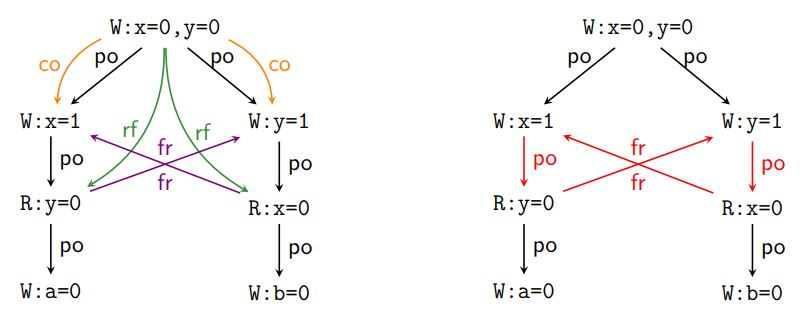
\includegraphics[scale=0.45]{includes/Figures/SCgraph.jpg}
	\end{figure}
	\item \po{} and \fr{} form a cycle
\end{itemize}
\end{frame}

\begin{frame}{Related Work}
\begin{itemize}
	\item KATER by \cite{Kok+23}
	\item KATI by \cite{Kou+24}
	\item RAT CAT SAT by \cite{Gru+26}
\end{itemize}
\end{frame}

\begin{frame}{The Proof System}
\begin{itemize}
	\item Produces implications of the form $\true \impl M_1 \subseteq M_2$ to prove this inclusion
	\item Start at the bottom with the inclusion term
	\item Transforms the inclusion and branches out to end at (possibly multiple) leafs which are \true 
%	\item[] \begin{figure} \small
%	\begin{mathpar}
%		\inferrule*[]{
%			\inferrule*[]{
%				\inferrule*[]{
%					\inferrule*[]{
%						\inferrule*[]{true}{\dots}
%					}{\dots}
%					\\
%					\inferrule*[]{
%						\inferrule*[]{true}{\dots}
%					}{\dots}				
%				}{\relr \subseteq \Rels}			
%			}{\dots}
%		}{M_1 \subseteq M_2}
%	\end{mathpar}
%	\end{figure}
\end{itemize}
\end{frame}

\begin{frame}{The Proof System}
\begin{itemize}
	\item Every one of the constraints can be transformed into any other
%	\begin{itemize}
%		\item[] \begin{rules}{Constraint Transformation}
%\inferrule*[left=($a\rightarrow i$)]{\texttt{irreflexive}~ \sf r^+}{\texttt{acyclic}~ \sf r} \and
%\inferrule*[left=($e \rightarrow i$)]{\texttt{irreflexive}~ \sf r.r^{-1}}{\texttt{empty}~ \sf r} \and
%\inferrule*[left=($i \rightarrow e$)]{\texttt{empty}~ \sf r \cap \id}{\texttt{irreflexive}~ \sf r} \and
%\inferrule*[left=($e \rightarrow a$)]{\texttt{acyclic}~ \sf r\cup r^{-1}}{\texttt{empty}~ \sf r}
%\end{rules}  
%	\end{itemize}
	\item Constraints can be eliminated when they are the same on both sides \\
%	\begin{rules}{Constraint Elimination} 
%\inferrule*[left=(empty)] {\sf r_1 \subseteq r_2}{\sf \texttt{empty}~ r_2 \subseteq \sf \texttt{empty}~ r_1} \and 
%\inferrule*[left=(acyclic)] {\sf r_1 \subseteq r_2}{\sf \texttt{acyclic}~ r_2 \subseteq \texttt{acyclic}~ r_1} \and
%\inferrule*[left={(irreflexive)}] {\sf r_1 \subseteq r_2}{\sf \texttt{irreflexive}~ r_2 \subseteq \texttt{irreflexive}~ r_1}
%\end{rules}
	
\end{itemize}
\end{frame}

\begin{frame}{Soundness}

\end{frame}

\begin{frame}{Completeness}

\end{frame}

\begin{frame}{Completeness}

\end{frame}

\begin{frame}{Evaluation}

\end{frame}

\begin{frame}{Conclusion}

\end{frame}

\begin{frame}{References}
\renewcommand{\bibfont}{\small}
\printbibliography
\end{frame}
\end{document}
